\documentclass{article}


\usepackage{latexsym}
\usepackage{graphicx}
\usepackage{amsmath}
\usepackage[fontset=mac]{ctex}
\usepackage{amsthm,amsmath,amssymb}
\usepackage{mathrsfs}

\title{NumPDEs}
\author{欧阳尚可  3190102458}
\date{\today}

\begin{document}
\maketitle
\newpage

\subsection*{Ex 10.159}
\indent 由图像可得其长度可表示为$L=U^{n+1}-u(t_{n+1})+u(t_n)-U^n$,而对于modified Euler method有$\Phi(U^n,t_n;k)=f(U^n+\frac{k}{2}f(U^n,t_n),t_n+\frac{k}{2})$。因此有$\mathcal{L}u(t_n)=u(t_{n+1})-u(t_n)-k\Phi(u(t_n)+\frac{k}{2}f(u(t_n),t_n),t_n+\frac{k}{2})= -L$。

\subsection*{Ex 10.161}
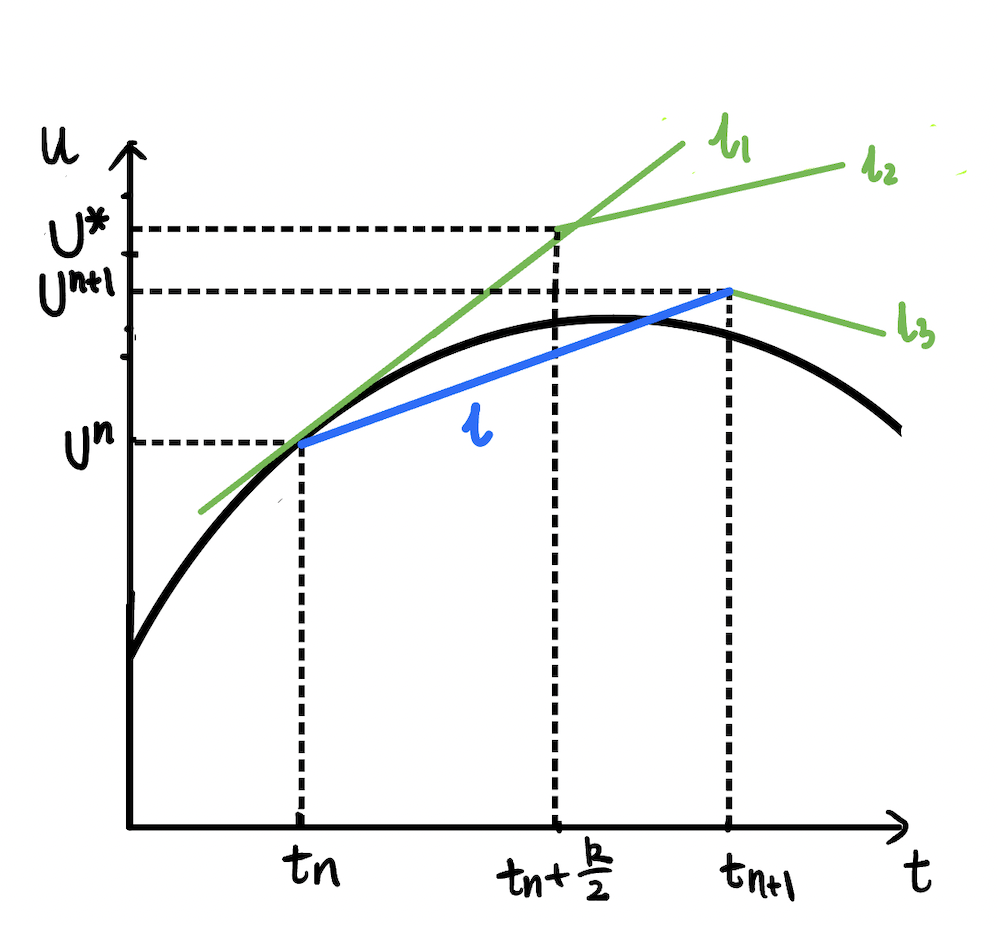
\includegraphics[scale = 0.6]{Ex161.png}

\subsection*{Ex 10.165}
\indent 我们使用Example 10.156中相同的记号。我们有
$$
\mathcal{L}u(t_n)=u(t_{n+1})-u(t_n)-ky_2=u(t_{n+1})-u(t_n)-kf(u(t_n)+\frac{k}{2}f,t_n+\frac{k}{2})
$$
有Taylor展开有
$$
f(u(t_n)+\frac{k}{2}f,t_n+\frac{k}{2})=f+\frac{k}{2}ff_u+\frac{k}{2}f_t+\frac{k^2}{8}f^2f_{uu}+\frac{k^2}{8}f_{tt}+\frac{k^2}{8}ff_{ut}+\frac{k^2}{8}ff_{tu}+O(k^3)\\
$$
$$
u(t_{n+1})-u(t_n)=kf+\frac{k^2}{2}(f_uf+f_t)+\frac{k^3}{6}(f_u^2f+f_{uu}f^2+f_uf_t+f_{tu}f+f_{ut}f+f_{tt})+O(k^4)
$$
由上面两式我们可以得到$\mathcal{L}u(t_n)=\Theta(k^3)$。

\subsection*{Ex 10.174}
\indent 我们考虑$u^{'}(t)=\lambda u$,由TR-BDF2的定义有
$$
U^{*}=U^n+\frac{k\lambda}{4}(U^n+U^{*})
$$
$$
U^{n+1}=\frac{1}{3}(4U^{*}-U^n+k\lambda U^{n+1})
$$
令$z=k\lambda$由第一个等式可以解得$U^{*}=\frac{1+\frac{z}{4}}{1-\frac{z}{4}}$再将结果带入第二个等式可以解得$U^{n+1}=\frac{1+\frac{5}{12}z}{1-\frac{7}{12}z+\frac{1}{12}z^2}$。\\
\indent 而对于$e^z$进行Taylor展开有$e^z=1+z+\frac{z^2}{2}+O(z^3)$因此$R(z)-e^z=\frac{5z^3-z^4}{24-14z+2z^2}+O(z^3)\rightarrow O(z^3),z\rightarrow0$。

\subsection*{Ex 10.179}
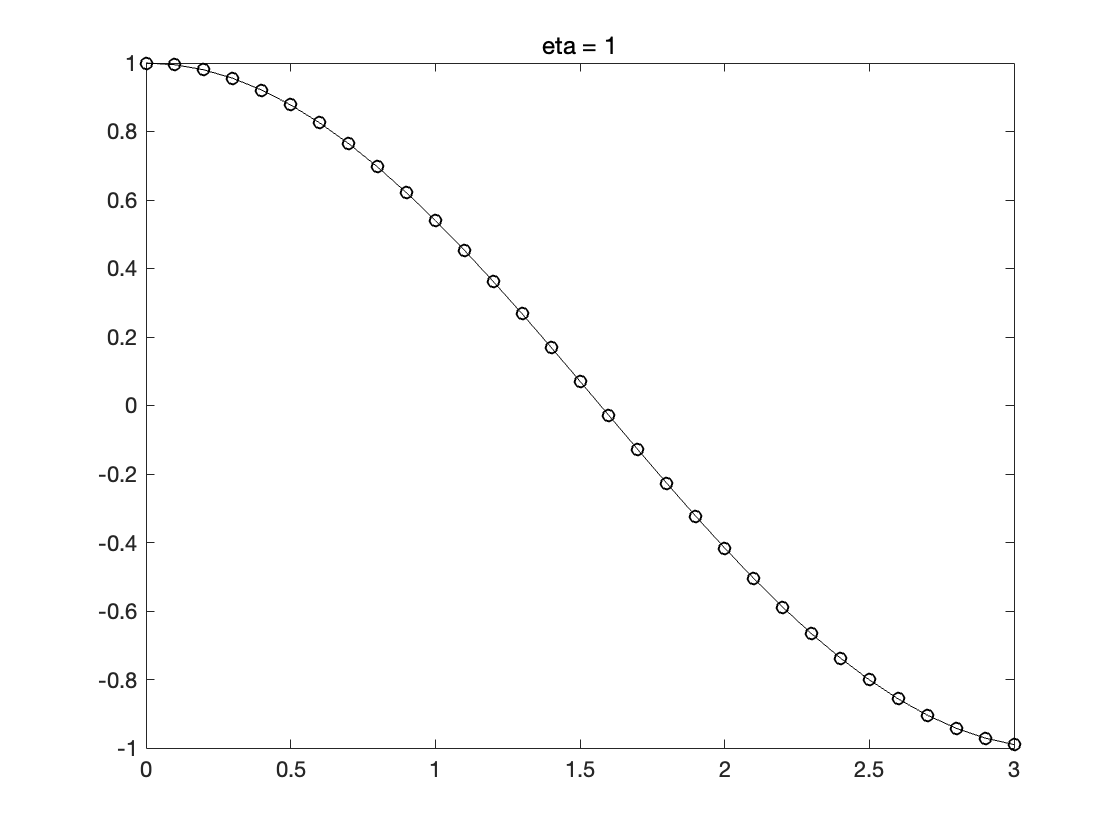
\includegraphics[scale = 0.125]{Ex179_1.png}
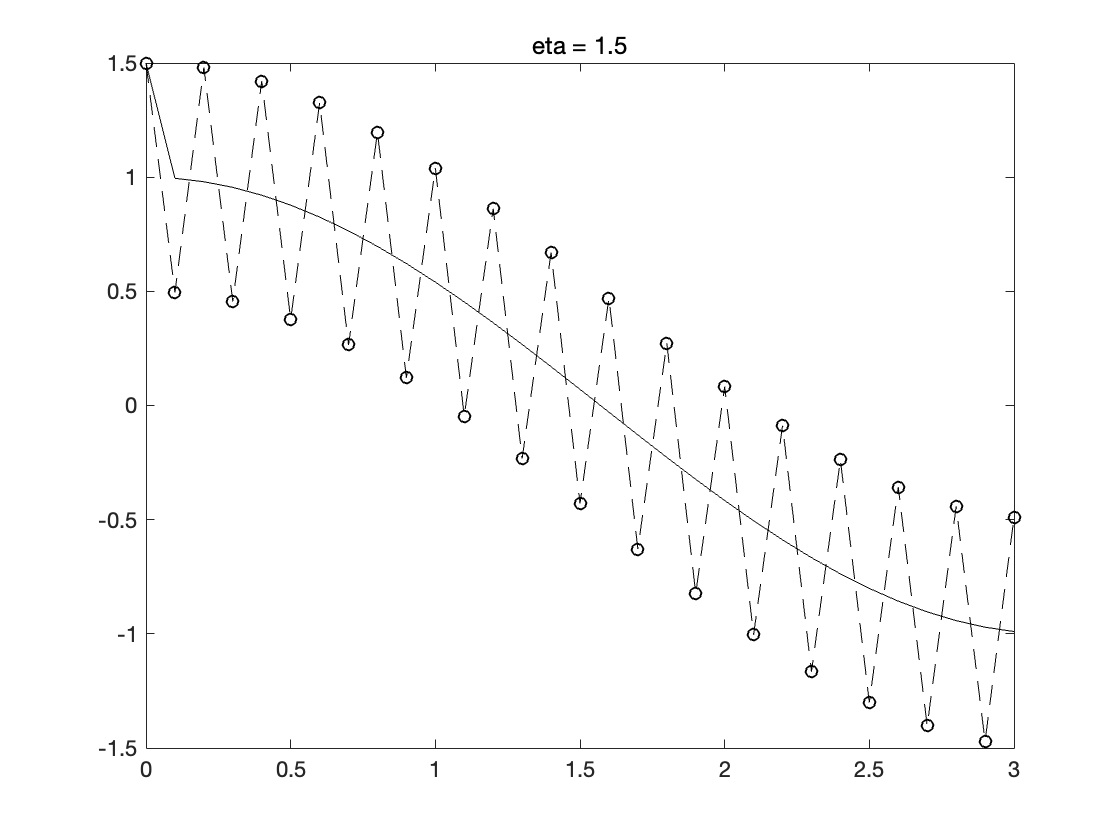
\includegraphics[scale = 0.125]{Ex179_2.png}

\subsection*{Ex 10.182}
\indent 由这三种方法定义不难得出

\begin{minipage}{\textwidth}
\begin{minipage}[t]{0.48\textwidth}
\makeatletter\def\@captype{table}
\begin{tabular}{c|c c}
    0 & 0 & 1 \\
    $\frac{1}{2}$ & $\frac{1}{2}$ & 0 \\
    \hline
    & 0 & 1
\end{tabular}
\caption{Modified Euler}
\label{sample-table}
\end{minipage}
\begin{minipage}[t]{0.48\textwidth}
\makeatletter\def\@captype{table}
\begin{tabular}{c|c c}
    0 & 0 & 0 \\
    1 & 1 & 0 \\
    \hline
    & $\frac{1}{2}$ & $\frac{1}{2}$
\end{tabular}
\caption{Improved Euler}
\label{sample-table}
\end{minipage}

\begin{minipage}[t]{\textwidth}
\makeatletter\def\@captype{table}
\begin{center}
\begin{tabular}{c|c c c}
    0 & 0 & 0 & 0\\
    $\frac{1}{3}$ & $\frac{1}{3}$ & 0 & 0 \\
    $\frac{2}{3}$ & 0 & $\frac{2}{3}$ & 0 \\
    \hline
    & $\frac{1}{4}$ & 0 & $\frac{3}{4}$
\end{tabular}
\end{center}
\caption{Heun's third-order}
\label{sample-table}
\end{minipage}

\end{minipage}

\subsection*{Ex 10.183}
\indent 为了简洁起见,我们记$y_i=f(\xi_i,t_n+c_ik)$。由此我们得到$\xi_i = U^n+k\sum_{j=1}^sa_{i,j}y_j$,带入第二个等式得到$U^{n+1}=U^n+k\sum_{j=1}^sb_jf(\xi_j,t_n+c_jk)=U^n+k\sum_{j=1}^sb_jf(U^n+k\sum_{l=1}^sa_{j,l}y_l,t_n+c_jk)$。由(10.121)中的第一个等式我们进一步得到:原式=$U^n+k\sum_{j=1}^sb_jy_j$这就是(10.121)中的第二个等式。

\subsection*{Ex 10.190}
\indent 由Taylor展开得到
\begin{equation*}
  \begin{aligned}
    	u(t_{n+1})-u(t_{n})&=kf+\frac{k^2}{2}(f_{u}f+f_{t})+\frac{k^3}{6}(f_{u}^{2}f+f_{uu}f^2+f_{u}f_{t}+f_{tu}f+f_{ut}f+f_{tt})+O(k^4)\\
	y_1&=f\\
	y_2&=f(U^n+ka_{21}y_1,t_n+c_2k)\\
	     &=f+k(a_{21}y_1f_u+c_2f_t)+\frac{k^2}{2}\{(a_{21}y_1)^2f_{uu}+a_{21}c_2y_1f_{ut}+a_{21}c_2y_1f_{tu}+c_2^2f_{tt}\}+O(k^3)\\
	y_3&=f(U^n+ka_{31}y_1+ka_{32}y_2,t_n+c_3k)\\
	     &=f+k[(a_{31}y_1+a_{32}y_2)f_u+c_3f_t]\\
	     &+\frac{k^2}{2}[(a_{31}y_1+a_{32}y_2)^2f_{uu}+c_3(a_{31}y_1+a_{32}y_2)f_{ut}+c_3(a_{31}y_1+a_{32}y_2)f_{tu}+c_3^2f_{tt}]+O(k^3)
  \end{aligned}
\end{equation*}
考虑到$\mathcal{L}u(t_n)=u(t_{n+1})-u(t_n)-kb_1y_1-kb_2y_2-kb_3y_3$。将上面展开的结果带入并且令$k,k^2,k^3$到系数全部为零并且运用等式$c_2=a_{21};c_3=a_{31}+a_{32}$
\begin{equation*}
\left\{
\begin{aligned}
1-b_1-b_2-b_3=0\\
\frac{1}{2}-b_2a_{21}-b_3(a_{31}+a_{32})=0\\
\frac{1}{3}-b_2a_{21}^2-b_3(a_{31}+a_{32})^2=0\\
\frac{1}{6}-b_3a_{21}a_{32}=0
\end{aligned}
\right.
\end{equation*}
题目中提到的一种形式只需要令$b_1=\frac{1}{4};b_3=\alpha$即可。

\subsection*{Ex 10.196}
($\Leftarrow$)由于f的阶数比r小,由Taylor展开有$f(t_n+c_jk)=f(t_{n})+c_jkf^{'}(t_n)+...+\frac{(c_jk)^(r-1)}{(r-1)!}f^{r-1}(t_n)$,再由$\sum_{j=1}^sb_jc_j^{l-1}=\frac{1}{l}$
\begin{equation*}
\begin{aligned}
k\sum_{j=1}^sb_jf(t_n+c_jk)&=k\sum_{j=1}^sb_j(f(t_n)+c_jkf^{'}(t_n)+...+\frac{(c_jk)^{r-1}}{(r-1)!}f^{r-1}(t_n))\\
	&=kf(t_n)+...+\frac{k^r}{r!}f^{r-1}(t_n)=\int_{t_n}^{t_n+k}f(t)dt
\end{aligned}
\end{equation*}
($\Rightarrow$)依题意得
\begin{equation*}
\begin{aligned}
I_s(f)&=k\sum_{j=1}^sb_jf(t_n+c_jk)=\int_{t_n}^{t_n+k}f(t)dt=kf(t_n)+...+\frac{k^r}{r!}f^{r-1}(t_n)\\
&\Rightarrow \forall l = 1,2,...,r,\sum_{j=1}^sb_jc_j^{l-1}=\frac{1}{l}
\end{aligned}
\end{equation*}

\subsection*{Ex 10.211}
\indent 由Definition 10.209我们知道
$$
u^{'}(t)-p^{'}(t)=\frac{u^{s+1}(\xi)}{s!}\prod_{i=1}^s(t-t_n-c_ik)
$$
记$M_i=max\{|c_i|,|1-c_i|\}$,我们有$|t-t_n-c_ik|\le M_ik$,再令$M=max_{t_n\le t\le t_{n+1}}\frac{u^{s+1}(t)}{s!}\prod_{i=1}^kM_i$我们可以得到$max_{t_n\le t\le t_{n+1}}|u^{'}(t)-p^{'}(t)|\le Mk^s$。再令$p(t_n)=u(t_n)$
\begin{equation*}
\begin{aligned}
|\mathcal{L}u(t_n)|=|u(t_{n+1})-p(t_{n+1})|=\int_{t_n}^{t_{n+1}}|u^{'}(t)-p^{'}(t)|dt\le Mk^{s+1}=O(k^{s+1})
\end{aligned}
\end{equation*}

\subsection*{Ex 10.213}
\indent 由$\forall i=1,2,...,s; \sum_{j=1}^sl_j(c_j)=1$且$\sum_{j=1}^sl_j(\tau)$小于s,故$\sum_{j=1}^sl_j(\tau)=1$,因此$\forall i=1,2,...,s$有
\begin{equation*}
\begin{aligned}
\sum_{j=1}^sa_{ij}=\int_0^{c_i}\sum_{j=1}^sl_j(\tau)d\tau=c_i\\
\sum_{j=1}^sb_j=\int_0^1\sum_{j=1}^sl_j(\tau)d\tau = 1
\end{aligned}
\end{equation*}

\subsection*{Ex 10.215}
\indent 仿照Example 10.214我们得到
\begin{equation*}
\begin{aligned}
l_1(\tau)=(2\tau-1)(4\tau-3)\\
l_2(\tau)=-(4\tau-1)(4\tau-3)\\
l_3(\tau)=(4\tau-1)(2\tau-1)
\end{aligned}
\end{equation*}
由(10.149)我们可以得到
\begin{center}
\begin{tabular}{c|c c c}
    $\frac{1}{4}$ & $\frac{23}{48}$ & -$\frac{1}{3}$ & $\frac{5}{48}$\\
    $\frac{1}{2}$ & $\frac{7}{12}$ & $-\frac{1}{6}$ & $\frac{1}{12}$ \\
    $\frac{3}{4}$ & $\frac{9}{16}$ & 0 & $\frac{3}{16}$ \\
    \hline
    & $\frac{2}{3}$ & $-\frac{1}{3}$ & $\frac{2}{3}$
\end{tabular}
\end{center}

\subsection*{Ex 10.218}
\indent 依题意得
\begin{equation*}
\begin{aligned}
(V\textbf{u})_k&=\sum_{j=1}^sc_j^{k-1}u_j=\sum_{j=1}^sc_j^{k-1}\sum_{i=1}^sb_ic_i^{m-1}a_{ij}=\sum_{i=1}^sb_ic_i^{m-1}\sum_{i=1}^sc_j^{k-1}a_{ij}\\
			&=\sum_{i=1}^sb_ic_i^{m-1}\frac{c_i^k}{k}=\frac{1}{k(m+k)}\\
(V\textbf{v})_k&=\sum_{j=1}^sc_j^{k-1}u_j=\sum_{j=1}^sc_j^{k-1}\frac{1}{m}b_j(1-c_j^m)=\frac{1}{mk}-\frac{1}{m(m+k)}=\frac{1}{k(m+k)}
\end{aligned}
\end{equation*}
这意味着V(\textbf{u}-\textbf{v})=0,而V为Vandermonde矩阵可以$\textbf{u}=\textbf{v}$。

\subsection*{Ex 10.222}
\indent 依题意得Ex 10.215中的方法是3-stage以及$q(x)=(x-\frac{1}{4})(x-\frac{1}{2})(x-\frac{3}{4})$,有$\int_0^kq(x)dx=0;\int_0^kq(x)xdx\ne0$可知他是四阶精确的。

\subsection*{Ex 10.248}
\indent 由定义得
$$
A=\left[ \begin{array}{c c c c}
0 & & & \\
\frac{1}{2} & 0 & & \\
0 & \frac{1}{2} & 0 & \\
0 & 0 & 1 & 0
\end{array}
\right]
$$
由此可得
$$
(I-zA)^{-1}=\left[ \begin{array}{c c c c}
1 & & & \\
\frac{z}{2} & 1 & & \\
\frac{z^2}{4} & \frac{z}{2} & 1 & \\
\frac{z^3}{4} & \frac{z^2}{2} & z & 1
\end{array}
\right]
$$
$\textbf{b}=[\frac{1}{6},\frac{1}{3},\frac{1}{3},\frac{1}{6}]^{T}$有$R(z)=1+z\textbf{b}^T(I-zA)^{-1}\textbf{1}=1+z+\frac{z^2}{2}+\frac{z^3}{6}+\frac{z^4}{24}$

\subsection*{Ex 10.242}
\indent 由上面可知$R(z)=1+z+\frac{z^2}{2}+\frac{z^3}{6}+\frac{z^4}{24}=e^z+O(z^5)$再由Theorem 10.249可知其四阶精确进一步得到$\mathcal{L}u(t_n)=O(k^5)$。

\subsection*{Ex 10.253}
\indent $\forall z\in S_1,|1+z|\le 1$,因此有$|1+z+\frac{z^2}{2}|=\frac{1}{2}|(z+1)^2+1|\le \frac{1}{2}(|z+1|^2+1)\le1$,因此$S_1\subset S_2$。\\
\indent $\forall z\in S_2,|1+z+\frac{z^2}{2}|<1$,记$1+z+\frac{z^2}{2}=re^{i\theta}$有$z=\sqrt{2re^{i\theta}-1}-1$\\
\indent 更高阶的情况显然不成立,因为z=0.03+i1.2时得到$z\in S_3,z\notin S_4$。


\subsection*{Ex 10.259}
\indent 依题意得A-stable RK方法是L-stable$\Leftrightarrow$$\lim_{z\rightarrow\infty}|R(z)|=\lim_{z\rightarrow\infty}|\frac{P(z)}{Q(z)}|=0$。而$Q(z)$与$P(z)$都是多项式,所以$\lim_{z\rightarrow\infty}|\frac{P(z)}{Q(z)}|=0\Leftrightarrow degQ(z)<degP(z)$。

\subsection*{Ex 10.262}
\indent (10.189)告诉我们$b_1\textbf{1}=A\textbf{e}_1$,而A是非奇异的,有$b_1A^{-1}\textbf{1}=\textbf{e}_1\Rightarrow b_1\textbf{b}^TA^{-1}\textbf{1}=\textbf{b}^T\textbf{e}_1\Rightarrow\textbf{b}^TA^{-1}\textbf{1}=1$。由此我们得到$\lim_{z\rightarrow\infty}R(z)=\lim_{z\rightarrow\infty}(z\textbf{b}^T(I-zA)^{-1}\textbf{1})=1-\textbf{b}^TA^{-1}\textbf{1}=0$。

\subsection*{Ex 10.267}

\subsection*{Ex 10.276}
\indent 我们定义$\textbf{e}^{n}=U^{n}-V^{n}$有
\begin{equation*}
\begin{aligned}
<\textbf{e}^{n+1},\textbf{e}^{n+1}>&=<\textbf{e}^{n+1},\textbf{e}^{n+1}-\textbf{e}^{n}>+<\textbf{e}^{n+1},\textbf{e}^{n}>\\
&=<\frac{\textbf{e}^{n+1}+\textbf{e}^{n}}{2},\textbf{e}^{n+1}-\textbf{e}^{n}>+<\frac{\textbf{e}^{n+1}-\textbf{e}^{n}}{2},\textbf{e}^{n+1}-\textbf{e}^{n}>+<\textbf{e}^{n+1},\textbf{e}^n>\\
&=<\frac{(U^{n+1}+U^n)-(V^{n+1}-V^n)}{2},k(f(\frac{U^{n+1}+U^n}{2},t_n+\frac{k}{2})-f(\frac{V^{n+1}+V^n}{2},t_n+\frac{k}{2}))>\\
&+<\frac{\textbf{e}^{n+1}-\textbf{e}^{n}}{2},\textbf{e}^{n+1}-\textbf{e}^{n}>+<\textbf{e}^{n+1},\textbf{e}^n>\\
&\le<\frac{\textbf{e}^{n+1}-\textbf{e}^{n}}{2},\textbf{e}^{n+1}-\textbf{e}^{n}>+<\textbf{e}^{n+1},\textbf{e}^n>\\
&=\frac{1}{2}<\textbf{e}^{n+1},\textbf{e}^{n+1}>+\frac{1}{2}<\textbf{e}^n,\textbf{e}^n>
\end{aligned}
\end{equation*}
因此有$<\textbf{e}^{n+1},\textbf{e}^{n+1}>\le<\textbf{e}^n,\textbf{e}^n>\Rightarrow||U^{n+1}-V^{n+1}||\le||U^n-V^n||$。





\end{document}